\begin{pastexam}[label={px:ntust-114-ice-12}]{臺科大資工所 114 學年度 第 12 題}
（填空；每格 5 分）

(10\%) Conduct an inorder traversal and a postorder traversal of the following binary tree.

\begin{center}
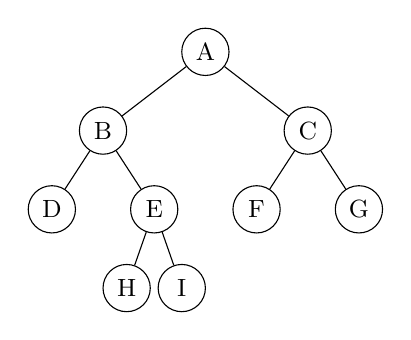
\begin{tikzpicture}[v/.style={circle,draw,minimum size=6mm,inner sep=0pt,font=\small}]
\node[v] (A) at (0,0) {A};
\node[v] (B) at (-1.3,-1) {B};
\node[v] (C) at (1.3,-1) {C};
\node[v] (D) at (-1.95,-2) {D};
\node[v] (E) at (-0.65,-2) {E};
\node[v] (F) at (0.65,-2) {F};
\node[v] (G) at (1.95,-2) {G};
\node[v] (H) at (-1.0,-3) {H};
\node[v] (I) at (-0.3,-3) {I};
\draw (A)--(B) (A)--(C) (B)--(D) (B)--(E) (C)--(F) (C)--(G) (E)--(H) (E)--(I);
\end{tikzpicture}
\end{center}

What is the 6th element of the inorder traversal? \blank{B}\\
What is the 6th element of the postorder traversal? \blank{C}
\end{pastexam}

\begin{pastsoln}
答案：(B) A；(C) F。

從圖讀出：A 的左右孩子是 B、C；B 的是 D、E；C 的是 F、G；E 的是 H、I。 走訪的定義見資結書第~7.3~節。

\textbf{中序}（左、根、右）：先走完 A 的左子樹。 B 的左子樹只有 D；接著 B；再走 E 的子樹得 H、E、I。
左子樹是 D、B、H、E、I，然後是 A，再走右子樹 F、C、G：
\[
\text{D, B, H, E, I, \textbf{A}, F, C, G}.
\]
第 $6$ 個是 A。 （左子樹恰好 $5$ 個節點，所以根排第 $6$。）

\textbf{後序}（左、右、根）：左子樹 B 的部分是 D、H、I、E、B；右子樹 C 的部分是 F、G、C；最後是 A：
\[
\text{D, H, I, E, B, \textbf{F}, G, C, A}.
\]
第 $6$ 個是 F。
\end{pastsoln}
